\begin{figure*}[!t]
    \centering
    \begin{subfigure}[t]{0.85\linewidth} % contains the two plots in a single figure
        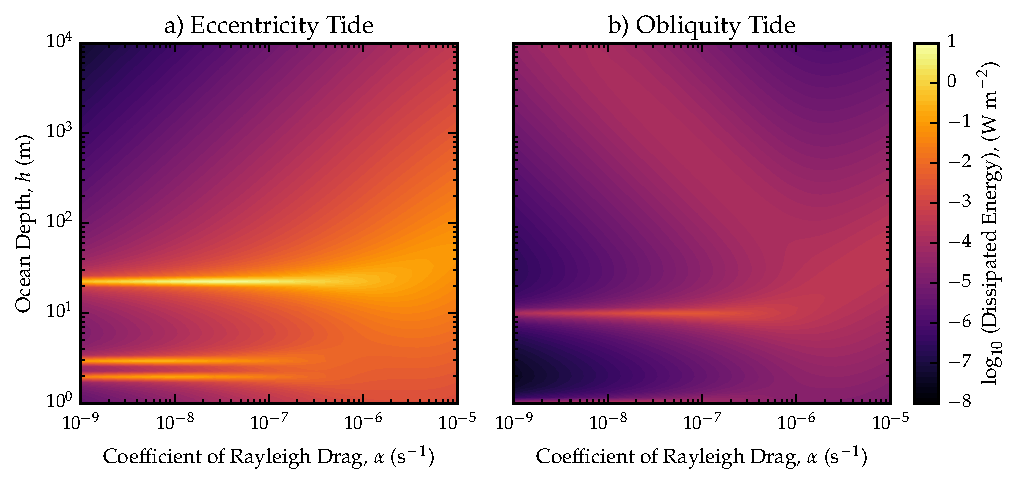
\includegraphics[width=\linewidth]{Figures/titan_linear}
        \phantomcaption
        \label{fig:lincEccTitan}
    \end{subfigure}
    \begin{subfigure}[t]{0\linewidth} % the hidden unwanted image
         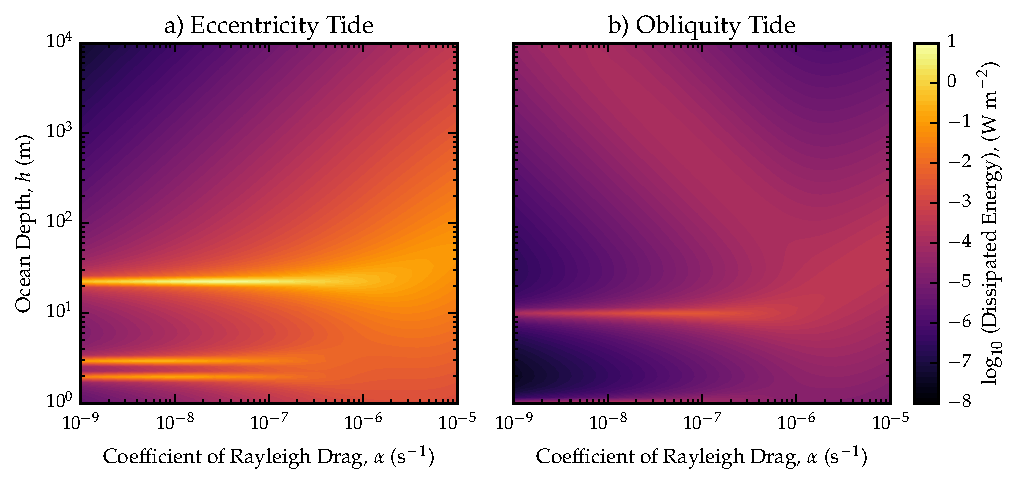
\includegraphics[width=\linewidth]{Figures/titan_linear}
         \phantomcaption
         \label{fig:linObliqTitan}   
    \end{subfigure}
    \vspace{-0.5cm}
\caption{Global ocean surface dissipation solution for Titan under the eccentricity (left) and obliquity (right) tides. The logarithm of dissipated energy is shown as a function of ocean depth, $h$, and Rayleigh drag coefficient, $\alpha$. All simulations were performed with \SIrange{2}{3}{\degree} resolution.}
\label{fig:linTitan}
\end{figure*}

\section{Ocean Dissipation in Titan \label{sec:results_Titan}}

The following results are split into three main sections. Firstly, we compare dissipation between Rayleigh (section \ref{sec:ray_titan}) and bottom (section \ref{subsec:botTitan}) drag for Titan. Section \ref{subsec:scalTitan} then compares the bottom drag results to scaling laws from \citet{chen2013tidal}. We repeat these results for Enceladus in section \ref{sec:results_Enceladus}.

\subsection{Rayleigh Drag}\label{sec:ray_titan}

Dissipated surface heat flux averaged over the tidal period was calculated for over 3000 simulations over $h$ and $\alpha$ space for each main tidal component, as shown in Figure \ref{fig:linTitan}. The eccentricity tide (Figure \ref{fig:lincEccTitan}) shows three resonant ocean thicknesses, $h \sim$ \SIlist{2;3;22}{\metre}. These horizontal resonances are the result of excited gravity waves, with the deepest of these having a maximum dissipated surface heat flux of $\sim 10\, \si{\watt\per\square\metre}$ which occurs between $\alpha =$ \SIrange{e-8}{e-7}{\per\second}. Notably, the maximum dissipated energy does not occur for the most drag dominated oceans where $\alpha \sim \num{e-5} \, \si{\per\second}$. 

\begin{figure*}[!t]
    \centering
    \begin{subfigure}[t]{0.85\linewidth} % contains the two plots in a single figure
        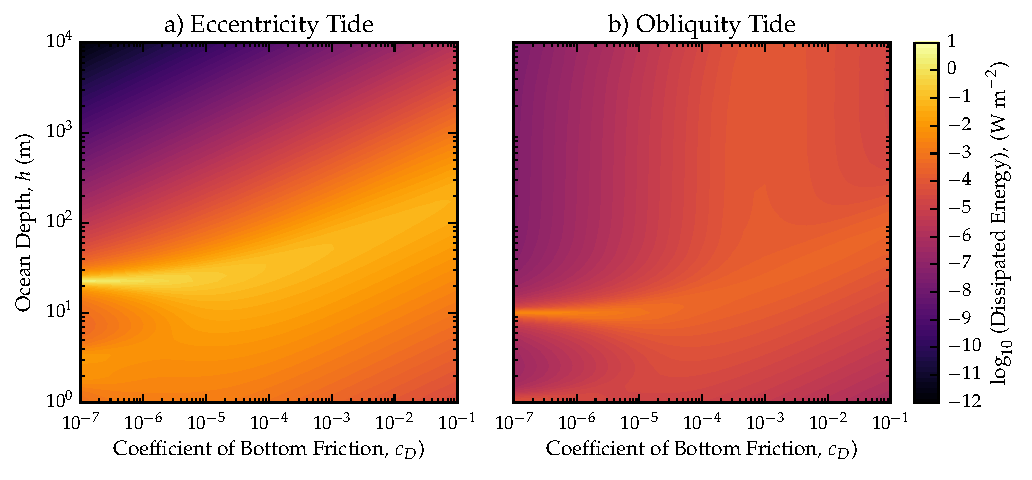
\includegraphics[width=\linewidth]{Figures/titan_bottom}
        \phantomcaption
        \label{fig:botEccTitan}
    \end{subfigure}
    \begin{subfigure}[t]{0\linewidth} % the hidden unwanted image
         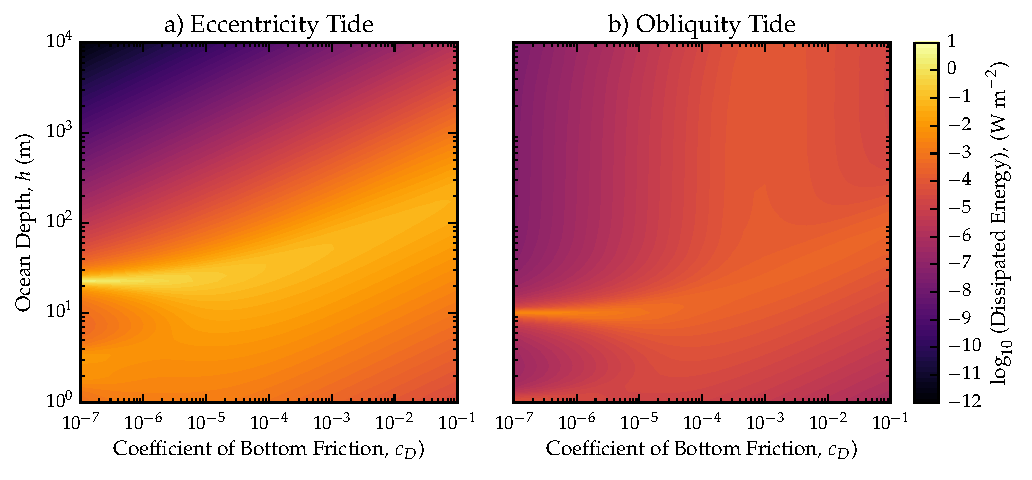
\includegraphics[width=\linewidth]{Figures/titan_bottom}
         \phantomcaption
         \label{fig:botObliqTitan}   
    \end{subfigure}
    \vspace{-0.5cm}
\caption{Global ocean surface dissipation solution for Titan under the eccentricity (left) and obliquity (right) tides. The logarithm of dissipated energy is shown as function of ocean depth, $h$, and coefficient of bottom drag, $c_D$. All simulations were performed with \SIrange{1}{3}{\degree} resolution. \label{fig:botTitan}}
\end{figure*}


Figure \ref{fig:linObliqTitan} illustrates the dissipated surface heat flux for the obliquity tide on Titan. Two resonant ocean thicknesses are found for this tidal component, $h \sim$ \SIlist{1;10}{\metre}. The latter resonance is the most dissipative with an average surface heat flux of $\sim \num{4e-3}\, \si{\watt\per\square\metre}$. There is also an excited Rossby wave resonance orientated diagonally across $h \sim$ \SIrange{10}{e4}{\metre} and \hbox{$\alpha \sim$ \SIrange{e-6}{e-9}{\per\second}}. The average surface heat flux occurring along the length of this resonance is $\sim \SI{e-4}{\watt\per\square\metre}$. 

Numerical error was also computed using the semi-analytical solutions from \citep{matsuyama2014tidal}. The eccentricity tide is accurate to within 1\% over much of the parameter space, with resonances being the least accurate (in terms of absolute value). The deepest resonance differs from the analytical solution by \SIrange{1}{20}{\percent}. We ignore discrepancies in shallow oceans ($h_0 \leq 10 \, \si{\metre}$) as bathymetry of the ocean floor for any icy satellite will likely be comparable to or exceed the depth of such a thin the ocean, directly violating the assumptions made in the LTEs. It should also be noted that resonances found below $h_0 = 10 \, \si{\metre}$ typical have displacements greater than the depth of the ocean itself, another violation of the LTEs assumptions. As such, we deem this part of the parameter space unphysical.

\subsection{Bottom Drag \label{subsec:botTitan}}

Dissipation across $h$ and $c_D$ space (bottom drag) is shown in Figure \ref{fig:botTitan}. Tidal dissipation due to the eccentricity tide is shown in the left hand figure. Comparing this to Rayleigh dissipation in Figure \ref{fig:lincEccTitan} highlights some of the major differences and similarities between the two drag regimes. The resonant peaks at \SIlist{2;3;22}{\metre} from the Rayleigh drag case are all present, although they have smaller magnitudes. The resonance broadens towards larger $c_D$, and remains very diffuse over much of the parameter space. This differs from the Rayleigh drag case where the resonances are very narrow and pronounced over most of $\alpha$ space (Figure \ref{fig:lincEccTitan}). Additionally, away from the resonances and in the deepest oceans, dissipated energy drops by \numrange{10}{12} orders of magnitude when applying bottom drag, which is far smaller than the lowest dissipation found in the Rayleigh drag case.  

Ocean dissipation under the obliquity tide using bottom drag also has several important differences and similarities to the Rayleigh case. Comparing figures \ref{fig:botObliqTitan} and \ref{fig:linObliqTitan}, it is again evident that the horizontal gravity wave resonances at \SIlist{1;10}{\metre} are present in both solutions. Perhaps the most significant difference between each case is the orientation of the broad resonance that extends to the deepest oceans. In the Rayleigh case, this resonance moves diagonally across a large region of the parameter space, whereas it is vertically oriented and limited to a small range of $c_D$ for the bottom drag case, such that the resonance becomes independent of ocean depth. The resonance also happens to occur across the empirically derived Earth value for $c_D = 0.002$ \citep[e.g.,][]{sohl1995tidal,egbert2001estimates}. %Unlike in the Rayleigh case, these resonances rapidly broaden towards higher $c_D$, when bottom drag becomes more dominant

\subsection{Comparison with Scaling Laws \label{subsec:scalTitan}}

\begin{figure*}[!t]
\centering
\begin{subfigure}{0.5\linewidth}
\centering
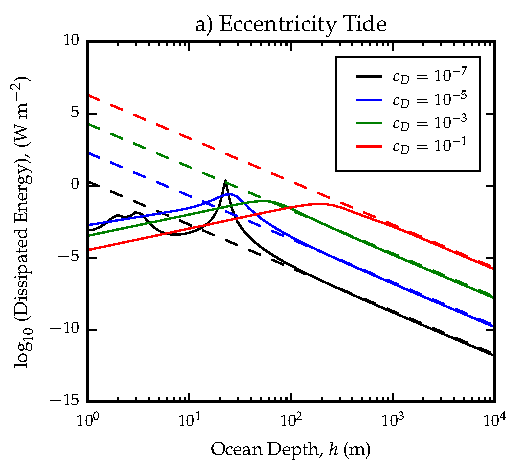
\includegraphics[width=0.85\linewidth]{Figures/Eccentricity_scaling}
\subcaption{\label{fig:scalEccTitan}}
\end{subfigure}%
\begin{subfigure}{0.5\linewidth}
\centering
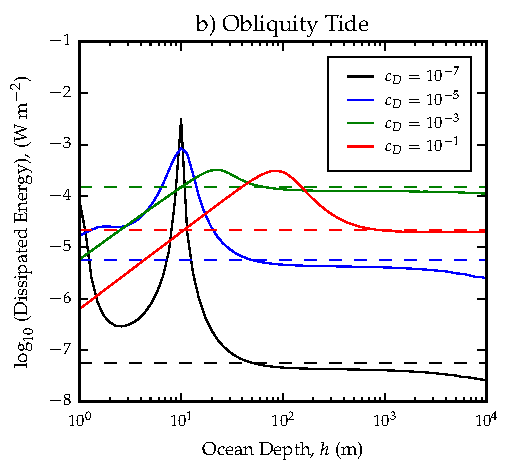
\includegraphics[width=0.85\linewidth]{Figures/Obliquity_scaling}
\subcaption{\label{fig:scalObliqTitan}}
\end{subfigure}
\vspace*{-0.8cm}
\caption{Comparison of the ODIS numerical results (solid lines) and those calculated using the scaling laws (dashed lines) derived in \citet{chen2013tidal}, for Titan under the eccentricity (left) and obliquity (right) tides. The colours represent different values of bottom drag coefficient.\label{fig:scalTitan}}
\end{figure*}

While there are no fully analytical solutions to the LTEs when including bottom drag, there are a set of scaling laws for estimating dissipation that neglect gravity wave resonant features, developed by \citet{chen2013tidal}. We compare cross sections from the results in Figure \ref{fig:botTitan} with these scaling laws, shown in Figure \ref{fig:scalTitan}.

Away from resonances and in deep oceans, there is excellent agreement between the numerical results and the scaling laws. This is particularly true of the eccentricity tide. Larger discrepancies are found for the obliquity tide (Figure \ref{fig:scalObliqTitan}) for deep oceans, but this is a result of discretisation error. The vertically orientated resonant feature in Figure \ref{fig:botObliqTitan} is also produced from the scaling laws, as shown in Figure \ref{fig:scalObliqTitan}. None of the gravity wave resonances are captured by the scaling laws. 

\subsection{Implications for Titan}

Titan likely has an ocean that is on the order of \SI{100}{\kilo\metre} thick \citep{sohl2014structural,baland2014titan}. All of the eccentricity tide resonances occur at ocean depths much shallower than this, suggesting that - despite the substantial free eccentricity - there is little dissipation from this tidal component in heating Titan's ocean.

Rossby wave resonances from the obliquity tide appear as the diagonal and vertical features in figures \ref{fig:linObliqTitan} and \ref{fig:botObliqTitan}, respectively. The linear drag resonance moves into unrealistically low Rayleigh drag coefficients ($\alpha \lesssim$ \SI{e-9}{\per\second}) for oceans deeper than about \SI{10}{\kilo\metre}. However, for bottom drag, the Rossby wave resonance is mainly independent of ocean depth above $h \gtrsim$ \SI{1}{\kilo\metre}. If Titan's ocean fell within the $c_D =$ \SIrange{e-2}{e-4} range then this Rossby wave resonance could provide a non-neglible thermal energy component to Titan's interior, regardless of the ocean depth. To gain some insight into how significant this dissipation can be, we consider some upper limits of Titan's semimajor axis evolution.

Hyperion is the next furthest satellite from Saturn after Titan, with a semimajor axis  \num{1.23} times that of Titan's (taken from the JPL satellite ephemerides: \url{http://ssd.jpl.nasa.gov/?sat_elem}). Titan would had to have originated at some semimajor axis less than Hyperion's, otherwise Hyperion would have been disturbed or ejected from the system, assuming Hyperion and Titan have similar ages. This provides us with a useful upper bound on Titan's  initial semimajor axis. Using the dissipated energy results for the obliquity tide under bottom drag we can examine how rapidly Titan's semimajor axis shrinks to its present day value.

For a bound orbit the total energy is given as $-GMm/2a$ \citep{murray1999solar}. Differentiating this expression with respect to time gives a relationship between the dissipated energy and changing semimajor axis,
\begin{equation}
\dot{a} = \dfrac{2a^2 \dot{E}}{GM m}.
\label{eq:adot}
\end{equation}

where $M$ and $m$ represent the mass of Saturn and Titan, respectively. The universal gravitational constant is $G$, and dissipated energy is $\dot{E}$. Note that as $\dot{E} < 0$, the semimajor axis decays with time. To first order, we find that $\dot{E}$ remains nearly constant over the range $1.21 a$ to $a$ for a deep ocean on Titan experiencing bottom drag for the obliquity tide. This is because the position of the vertical Rossby wave resonance (Figure \ref{fig:botObliqTitan}) is sensitive to the rotation rate of Titan, which hardly varies from $\Omega =$ \SIrange{4.56e-6}{3.42e-6}{\per\second} over the range of semimajor axes that we consider, assuming synchronous rotation. We are thus able to set $\dot{E}$ to constant in the following calculations. Additionally, it should be noted that while $\dot{E}$ is rather sensitive to the actual obliquity, $\theta_0$, we set the obliquity to constant over time for simplicity. A more rigorous (and future) approach would include the coupling between energy and obliquity.

\begin{figure}[!b]
\centering
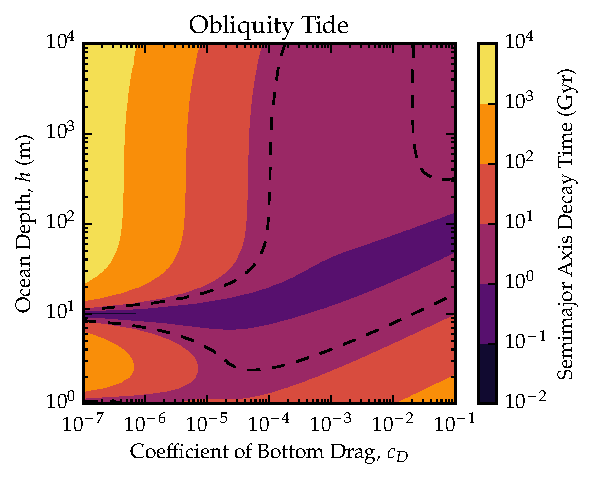
\includegraphics[width=\linewidth]{Figures/titan_timescale}
\caption{Semimajor axis decay timescale, $\tau_a$, as a function of ocean depth and bottom drag coefficient for the obliquity tide on Titan. This timescale represents the time taken for the semimajor axis of Titan to shrink from that of Hyperion's to the present day value. The dashed contour represents the age of the Solar System, $\sim \SI{4.5}{\giga\year}$. \label{fig:a_evo}}
\end{figure}

\begin{figure*}[!t]
    \centering
    \begin{subfigure}[t]{0.85\linewidth} % contains the two plots in a single figure
        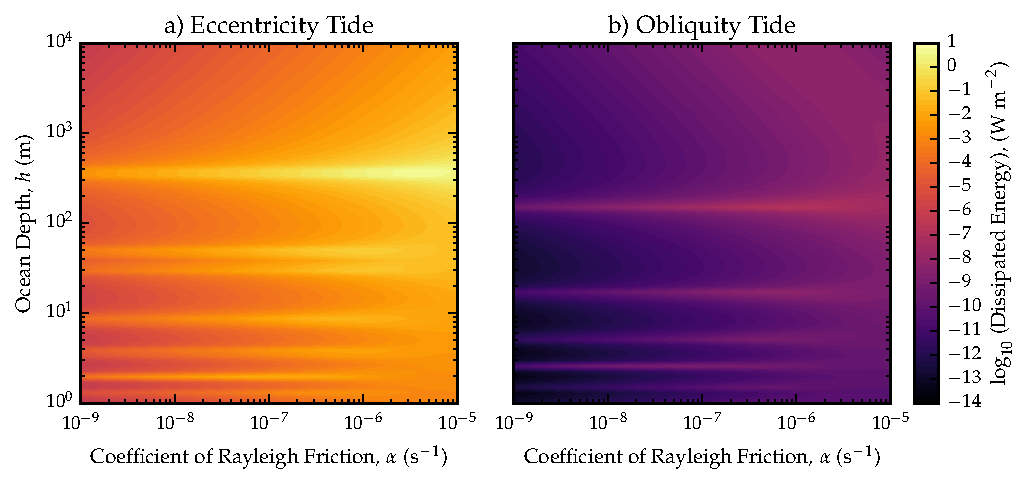
\includegraphics[width=\linewidth]{Figures/enceladus_linear}
        \phantomcaption
        \label{fig:lincEccEncel}
    \end{subfigure}
    \begin{subfigure}[t]{0\linewidth} % the hidden unwanted image
         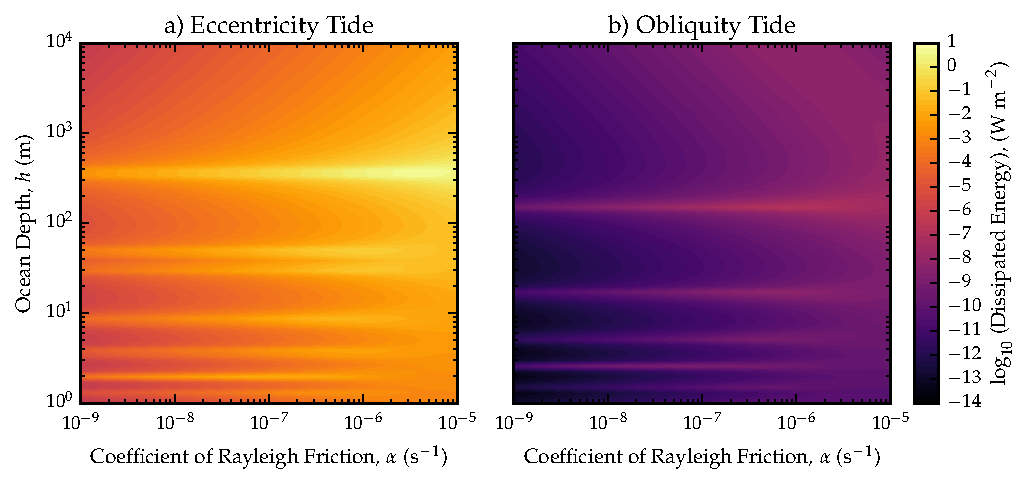
\includegraphics[width=\linewidth]{Figures/enceladus_linear}
         \phantomcaption
         \label{fig:linObliqEncel} 
    \end{subfigure}
    \vspace{-0.5cm}
\caption{Time and surface averaged ocean dissipation for Enceladus under the eccentricity (left) and obliquity (right) tides when applying Rayleigh drag. The logarithm of dissipated energy is shown as function of ocean depth, $h$, and bottom drag coefficient, $c_D$. All simulations were performed with \SIrange{1}{3}{\degree} grid resolution. \label{fig:linEncel}}
\end{figure*}

We integrate Equation \ref{eq:adot} to estimate the evolution of Titan's semimajor axis as a function of time and dissipated energy, defining a characteristic semimajor axis decay time, $\tau_{a}$, as the time taken for the semimajor axis to reach its present day value from Hyperion's. The decay time as a function of ocean depth and bottom drag coefficient is shown in Figure \ref{fig:a_evo}.
  
As expected, the smallest $\tau_a$ occurs for the largest dissipation, namely the gravity wave resonance at \SI{10}{\metre}, with decay times on the order of \SIrange{10}{100}{\mega\year}. However, as previously mentioned, Titan's ocean is likely in excess of \SI{100}{\kilo\metre} thick, and is thus far from this resonance. Figure \ref{fig:a_evo} shows that for ocean depths $h_0 >$ \SI{1}{\kilo\metre} the decay time-scale (and dissipation) is effectively independent of ocean depth. Although not shown, this behaviour continues right up to the shallow water limit ($h_0 \lesssim 0.1r$) as predicted by the \citet{chen2013tidal} scaling laws. Thus, for $c_D =$ \SIrange{e-4}{2e-2}, Titan's semimajor axis would shrink to its present day value in less than the age of the Solar System ($\sim$\SI{4.5}{\giga\year}, denoted by the dashed contour in Figure \ref{fig:a_evo}). If Titan's orbit originated with a semimajor axis between its current value and less than Hyperion's value, then we would expect Titan to have a smaller semimajor axis than that observed today.

Although the initial value of $a$ is not known, the scenario described above is not consistent with the deep ocean estimates of \citet{sohl2014structural, baland2014titan} if we assume a bottom drag coefficient within an order of magnitude of the canonical Earth value ($c_D =$ \num{0.002}). Instead, our estimates of the decay time-scale suggest that Titan's ocean has a bottom drag coefficient of \hbox{$ \num{e-4} \gtrsim c_D \gtrsim \num{2e-2} $}. These constraints indicate that Titan's ocean experiences anomalously low or high drag (not dissipation) than compared to the Earth's ocean.

Titan is a very slow rotator, resulting in limited ocean flow. This factor reduces the amount of turbulent bottom flow experienced in the ocean, consequently lowering the bottom drag coefficient. This is consistent with the low drag limit. However, one could additionally argue that the presence of a solid lid, although neglected here, would result in an extremely turbulent ``top'' drag environment, consistent with the high drag limit. At present there is not sufficient evidence to favour one of these limits over the other and should be a focus of future work.  

Although we do not attempt to compute the eccentricity evolution (which is far more challenging with non-radial tidal components), the almost negligible amount of dissipated energy for $h_0 >$ \SI{1}{\kilo\metre} shown in Figure \ref{fig:botObliqTitan} should allow Titan to maintain its relatively high free eccentricity of 0.0288. Here we of course neglect dissipation in Titan's solid interior.